\section{Experimento com BRDF Anisotrópica: Kajiya-Kay (1989)}

A BRDF de especularidade anisotrópica, baseada no trabalho seminal de @@REF Kajiya-Kay de 1989, modela a reflexão especular em superfícies com características direcionais, como tecidos e cabelos. Esta abordagem captura de forma
sofisticada a distribuição de luz em superfícies com orientação preferencial. As equações que descrevem esse experimento se encontram em \autoref{fig-kajiya-eqlang-latex}. O código fonte de entrada para o compilador está em \autoref{cod-kajiya-eqlang}. A redenrização de um objeto 3D usando essa BRDF esta em \autoref{fig-kajiya-eqlang}.

\subsection{Representação em documento \LaTeX{}}
\begin{figure}[H]
    \caption{\label{fig-kajiya-eqlang-latex} \small Equações da BRDF do experimento Kajiya-Kay em documento \LaTeX{}.}
    \begin{center}
        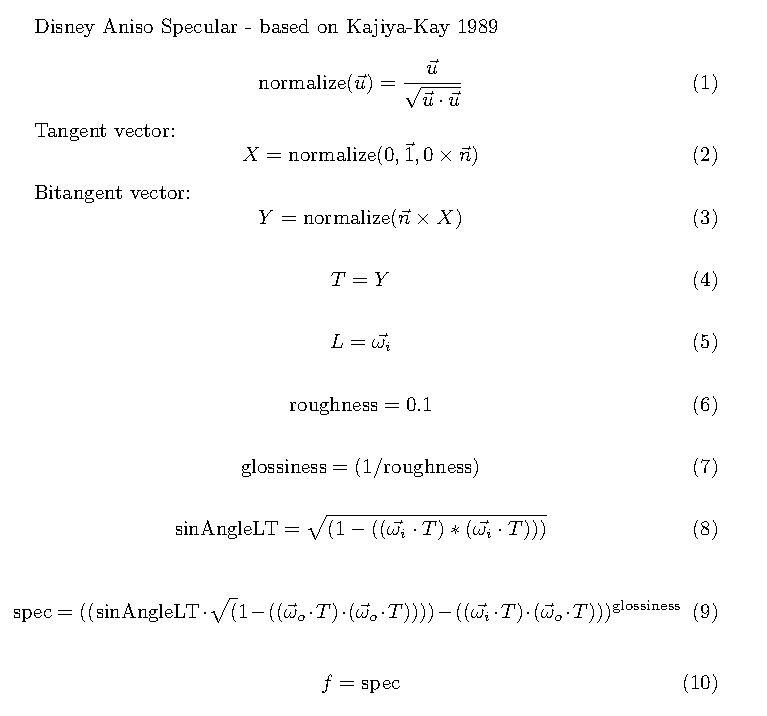
\includegraphics[scale=1.1,width=\textwidth]{./Imagens/brdfs/aniso.pdf}
        % 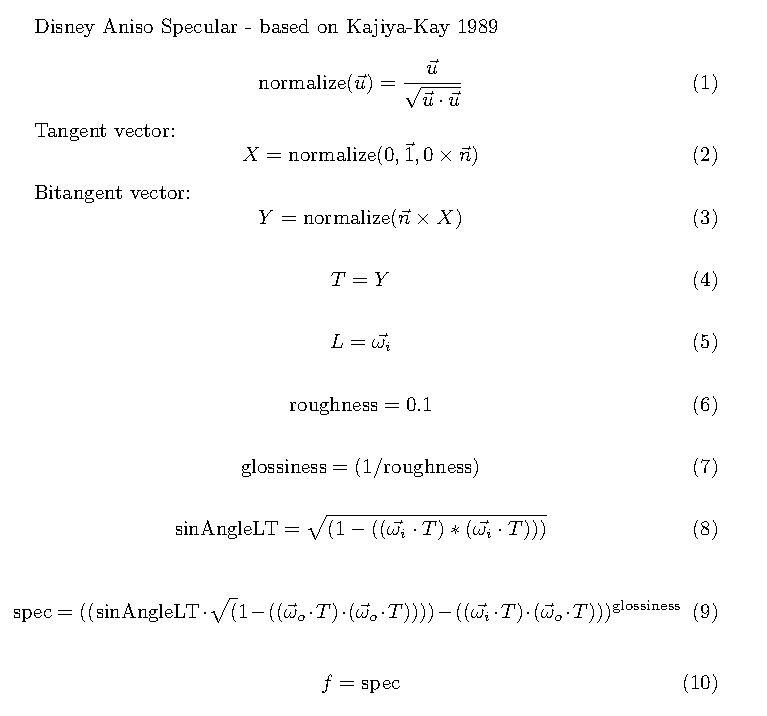
\includegraphics[scale=1.1]{./Imagens/brdfs/aniso.pdf}
    \end{center}
\end{figure}

% \begin{align}
%     \text{Vetores Fundamentais:} & \nonumber \\
%     \vec{X} &= \text{normalize}(\vec{0,1,0} \times \vec{n}) \\
%     \vec{Y} &= \text{normalize}(\vec{n} \times \vec{X}) \\
%     T &= \vec{Y} \\
%     \text{Parâmetros:} & \nonumber \\
%     \text{Rugosidade} &= 0.1 \\
%     \text{Brilho} &= (1/\text{Rugosidade}) \\
%     \text{Componente Especular:} & \nonumber \\
%     \text{spec} &= \left(\frac{\sin(\text{ângulo}_{\text{LT}}) \sqrt{1 - \cos^2(\text{ângulo}_{\text{VT}})}}{\cos(\text{ângulo}_{\text{LT}}) \cos(\text{ângulo}_{\text{VT}})} \right)^{\text{brilho}}
% \end{align}

\subsection{Código Fonte em \texttt{EquationLang}}
\begin{codigo}[H]
    \caption{\small Código fonte da BRDF do experimento Kajiya-Kay.}
    \label{cod-kajiya-eqlang}
\begin{lstlisting}[language=tex, frame=none, inputencoding=utf8]
    Disney Aniso Specular - based on Kajiya-Kay 1989
    \begin{equation}
      \text{normalize}(\vec{u}) = \frac{\vec{u}}{\sqrt{\vec{u} \cdot \vec{u}}}
    \end{equation}

    \begin{equation}
    reflect(\vec I, \vec N) =  2*(\vec I \cdot \vec N)*\vec N - \vec I
    \end{equation}

    Tangent vector:
    \begin{equation}
       X = \text{normalize}(\vec{0,1,0} \times \vec{n})
    \end{equation}

    Bitangent vector:
    \begin{equation}
       Y = \text{normalize}(\vec{n} \times X)
    \end{equation}

    \begin{equation}
        T = Y
    \end{equation}

    \begin{equation}
    roughness =  0.1
    \end{equation}

    \begin{equation}
        glossiness = (1/roughness)
    \end{equation}
    \begin{equation}
        lightAngle = (\vec{\omega_i} \cdot \vec{n})
    \end{equation}

    \begin{equation}
        cosAngleLT = (\vec{\omega_i} \cdot T)
    \end{equation}

    \begin{equation}
        sinAngleLT = \sqrt(1 - (cosAngleLT * cosAngleLT))
    \end{equation}

    \begin{equation}
        cosAngleVT = (\vec \omega_o \cdot T)
    \end{equation}

    \begin{equation}
    spec = ((sinAngleLT * \sqrt(1 - (cosAngleVT * cosAngleVT)))
                      - (cosAngleLT * cosAngleVT))^ glossiness
    \end{equation}

    \begin{equation}
    f = spec
    \end{equation}
\end{lstlisting}
\end{codigo}

\subsection{Código GLSL Gerado}

\begin{codigo}[H]
    \caption{\small Saida do compilador, código GLSL da BRDF do experimento Kajiya-Kay (parte 1). }
    \label{cod-kajiya-eqlang-declarations}
\begin{lstlisting}[language=C, inputencoding=utf8]
    
    analytic
    ::begin parameters
    # [type] [name] [min val] [max val] [default val]
    ::end parameters

    ::begin shader


    //////////// START OF BUILTINS DECLARTION ////////////
    vec3  var_0_vec_h;
    vec3  var_3_vec_n;
    float var_10_theta_h;
    float var_11_theta_d;
    float var_1_pi;
    float var_2_epsilon;
    vec3  var_4_vec_omega_i;
    float var_5_theta_i;
    float var_6_phi_i;
    vec3  var_7_vec_omega_o;
    float var_8_theta_o;
    float var_9_phi_o;
    //////////// END OF BUILTINS DECLARTION ////////////


    //////////// START OF USER DECLARED ////////////
    vec3  var_14_X;
    vec3  var_15_Y;
    vec3  var_16_T;
    float var_17_cosAngleLT;
    float var_18_cosAngleVT;
    float var_19_roughness;
    float var_20_glossiness;
    float var_21_sinAngleLT;
    float var_22_spec;
    float var_23_f;
    float var_27_lightAngle;
    //////////// END OF USER DECLARED ////////////

\end{lstlisting}
\end{codigo}

\begin{codigo}[H]
    \caption{\small Saida do compilador, código GLSL da BRDF do experimento Kajiya-Kay (parte 2). }
    \label{cod-kajiya-eqlang}
\begin{lstlisting}[language=C, inputencoding=utf8]
    //////////// START FUNCTIONS DECLARATIONS ////////////
    vec3 var_12_text_normalize(vec3 var_13_vec_u) {
        return (var_13_vec_u/sqrt(dot(var_13_vec_u,var_13_vec_u)));
    }
    vec3 var_24_reflect(vec3 var_25_vec_I, vec3 var_26_vec_N) {
        return (((2.0*(dot(var_25_vec_I,var_26_vec_N)))*var_26_vec_N)-var_25_vec_I);
    }
    //////////// END FUNCTIONS DECLARATIONS ////////////

    vec3 BRDF(vec3 L, vec3 V, vec3 N, vec3 X, vec3 Y ) {

    //////////// START OF BUILTINS INITIALIZATION ////////////
         var_0_vec_h = normalize(L+V);
         var_3_vec_n = normalize(N)  ;
         var_1_pi = 3.141592653589793 ;
         var_2_epsilon = 1.192092896e-07 ;
         var_4_vec_omega_i = L ;
         var_5_theta_i = atan(var_4_vec_omega_i.y,var_4_vec_omega_i.x) ;
         var_6_phi_i = atan(sqrt(var_4_vec_omega_i.y*var_4_vec_omega_i.y+var_4_vec_omega_i.x*var_4_vec_omega_i.x),var_4_vec_omega_i.z) ;
         var_7_vec_omega_o = V ;
         var_8_theta_o = atan(var_7_vec_omega_o.y,var_7_vec_omega_o.x) ;
         var_9_phi_o = atan(sqrt(var_7_vec_omega_o.y*var_7_vec_omega_o.y+var_7_vec_omega_o.x*var_7_vec_omega_o.x),var_7_vec_omega_o.z) ;
         var_10_theta_h = acos(dot( var_0_vec_h , N));
         var_11_theta_d = acos(dot( var_0_vec_h , var_4_vec_omega_i ));
    //////////// END OF BUILTINS INITIALIZATION ////////////

        var_14_X = var_12_text_normalize(cross(vec3(0.0, 1.0, 0.0),var_3_vec_n));
        var_15_Y = var_12_text_normalize(cross(var_3_vec_n,var_14_X));
        var_16_T = var_15_Y;
        var_17_cosAngleLT = (dot(var_4_vec_omega_i,var_16_T));
        var_18_cosAngleVT = (dot(var_7_vec_omega_o,var_16_T));
        var_19_roughness = 0.1;
        var_20_glossiness = ((1.0/var_19_roughness));
        var_21_sinAngleLT = sqrt(((1.0-((var_17_cosAngleLT*var_17_cosAngleLT)))));
        var_22_spec = pow(((((var_21_sinAngleLT*sqrt(((1.0-((var_18_cosAngleVT*var_18_cosAngleVT)))))))-((var_17_cosAngleLT*var_18_cosAngleVT)))),var_20_glossiness);
        var_23_f = var_22_spec;
        var_27_lightAngle = (dot(var_4_vec_omega_i,var_3_vec_n));

        return vec3(var_23_f);
    }
\end{lstlisting}
\end{codigo}



\subsection{Visualização do Resultado}
    \begin{figure}[h]
        \centering
        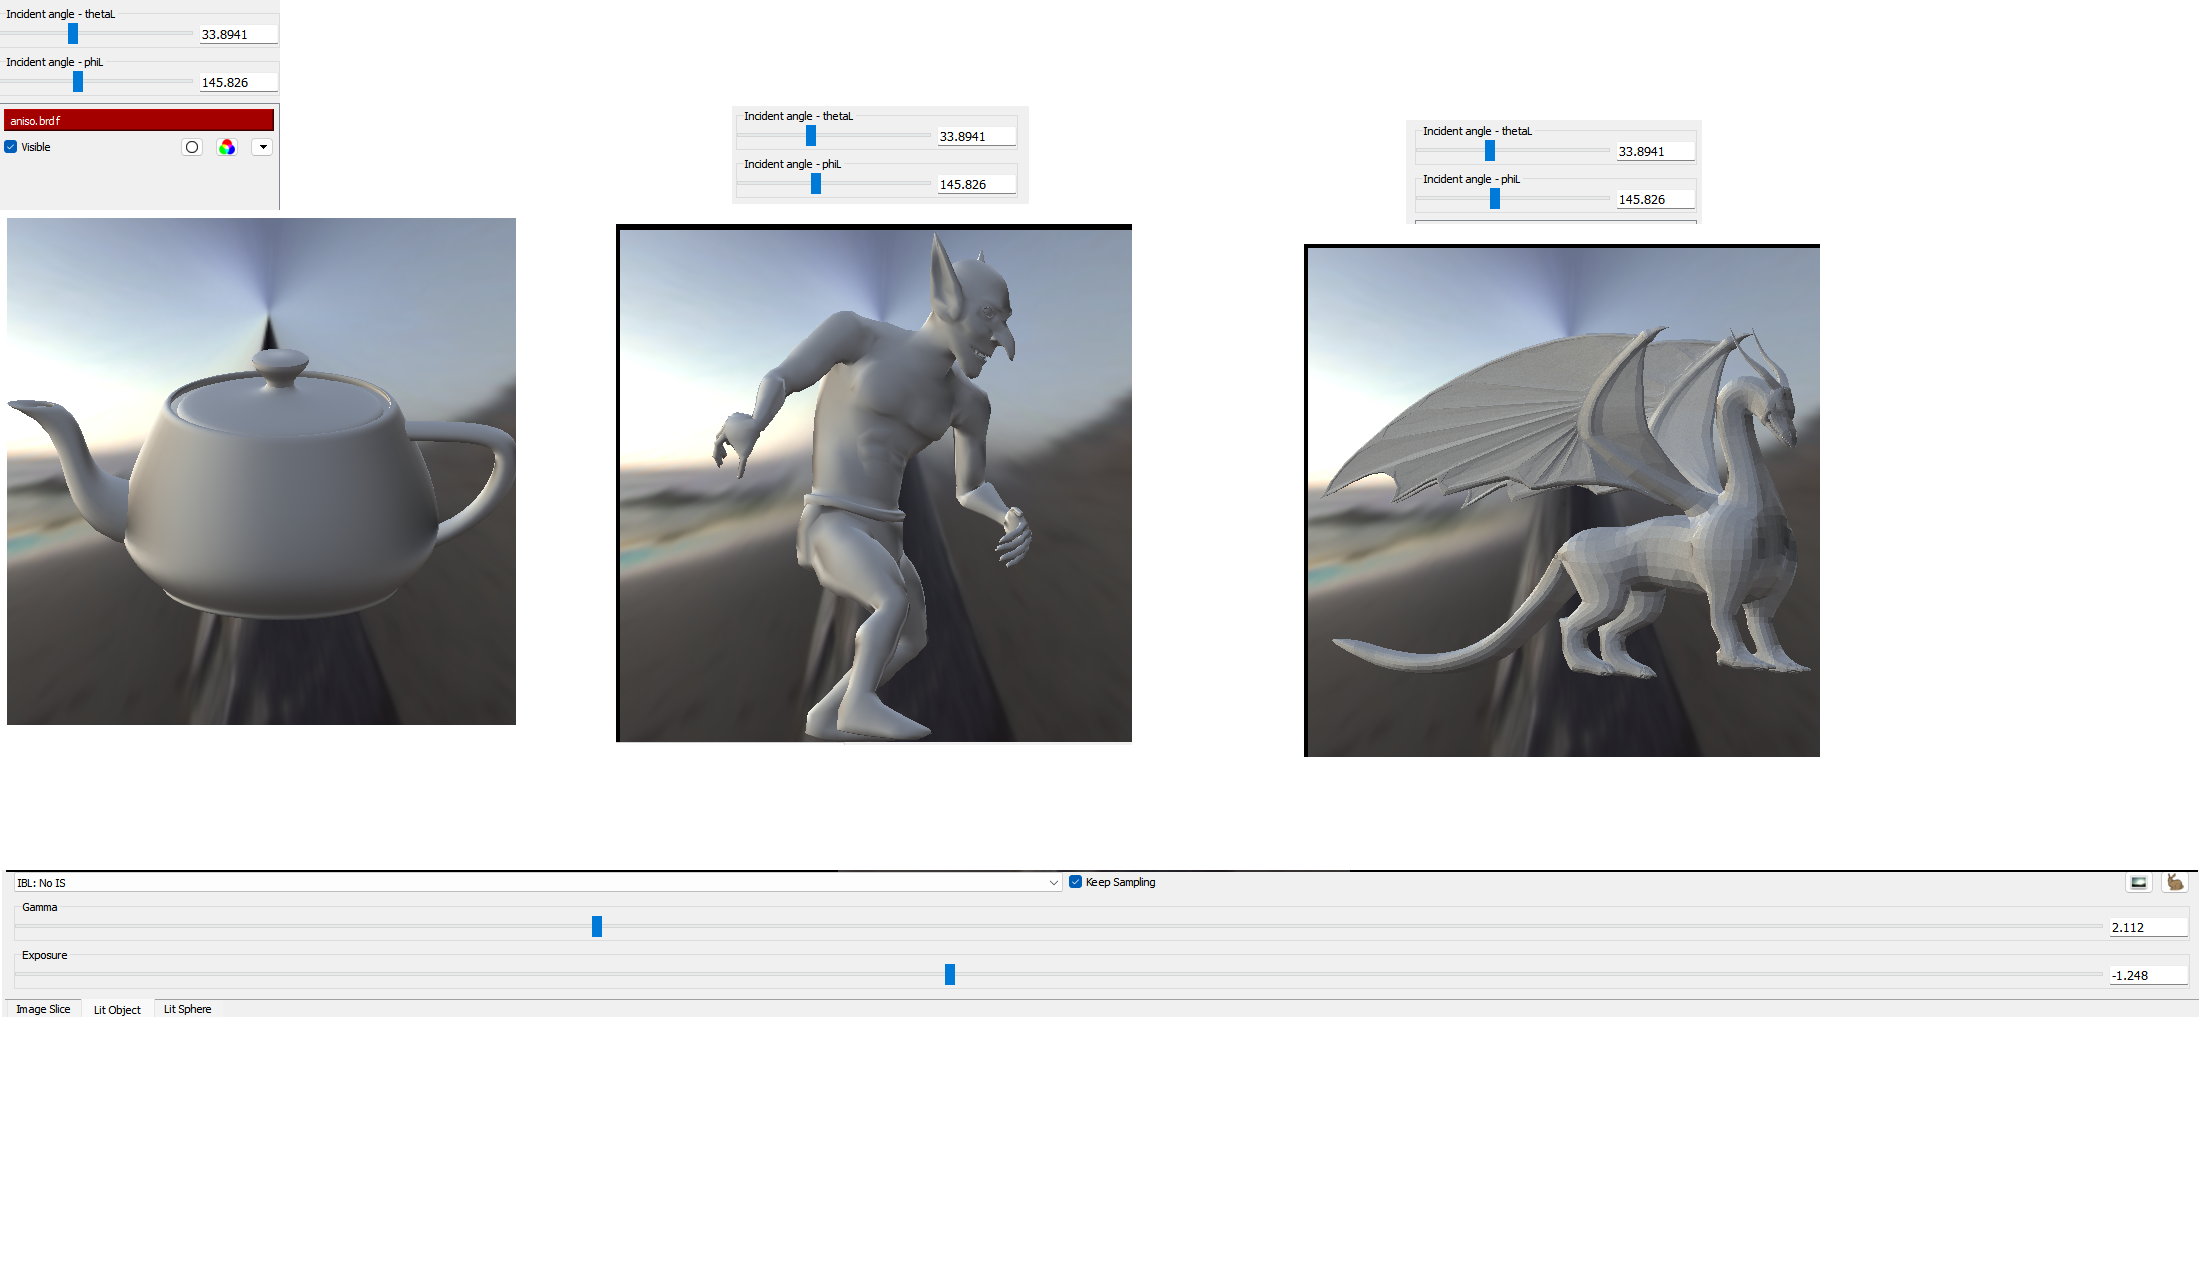
\includegraphics[scale=1.9, width=\textwidth]{Imagens/brdfs/aniso.png}
    \caption{Distribuição de Reflexão Especular da BRDF Anisotrópica de Disney}
    \label{fig:disney_anisotropic_specular}
\end{figure}
